\documentclass{article}
\usepackage{amsmath, amssymb, graphicx, booktabs}
\usepackage[margin=2.5cm]{geometry}
\usepackage{listings}
\usepackage{xcolor}
\usepackage{float}

\title{Report for the practical assignment
Automated Reasoning 2IMF25}
\author{
\begin{tabular}{c c c}
\multicolumn{3}{c}{Group 37}\\[1em]
Luxue Wen & Kaiwen Tan & Yan Liu\\
student number: 2271796 & student number: 2291797 & student number: 2176246\\
email: l.wen@student.tue.nl & email: k.tan@student.tue.nl &  email: y.liu17@student.tue.nl
\end{tabular}
}
\date{September, 2025}

\lstset{
    basicstyle=\ttfamily\small,
    keywordstyle=\color{blue},
    commentstyle=\color{green!60!black},
    stringstyle=\color{red},
    numbers=left,
    numberstyle=\tiny,
    breaklines=true,
    frame=single,
    columns=fullflexible
}

\begin{document}

\maketitle

\section*{Problem 1: Magic Factory}

\section{Modeling the Problem}

\subsection{Parameters}
\begin{itemize}
  \item $T = 8$: number of trucks.
  \item $C = 8000$: capacity (kg) per truck.
  \item $P = 8$: maximum number of pallets per truck.
  \item Pallet types:
    \begin{itemize}
      \item Nuzzles: 4 pallets, 700 kg each.
      \item Skipples: 8 pallets, 1000 kg each, require cooling.
      \item Crottles: 10 pallets, 2500 kg each.
      \item Dupples: 20 pallets, 200 kg each.
      \item Prittles: unlimited supply, 400 kg each (objective: maximize).
    \end{itemize}
  \item Cooling: only 3 trucks can carry skipples.
\end{itemize}

\subsection{Decision Variables}
Let:
\[
x_{i,t} \in \mathbb{N}
\]
be the number of pallets of type $i$ assigned to truck $t$, where $i \in \{\text{nuzzle}, \text{prittle}, \text{skipple}, \text{crottle}, \text{dupple}\}$ and $t \in \{1, \ldots, 8\}$.

Additionally:
\[
y_t \in \{0,1\}
\]
indicates whether truck $t$ is equipped with cooling (1) or not (0).

\subsection{Constraints}
\paragraph{Truck capacity (weight):}
\[
\forall t: \quad \sum_i (w_i \cdot x_{i,t}) \leq C
\]

\paragraph{Truck capacity (pallet count):}
\[
\forall t: \quad \sum_i x_{i,t} \leq P
\]

\paragraph{Supply limits:}
\[
\sum_t x_{\text{nuzzle},t} = 4, \quad
\sum_t x_{\text{skipple},t} = 8, \quad
\sum_t x_{\text{crottle},t} = 10, \quad
\sum_t x_{\text{dupple},t} = 20
\]

\paragraph{Cooling requirement:}
\[
\sum_t y_t = 3, \quad \forall t: x_{\text{skipple},t} \leq P \cdot y_t
\]

\paragraph{Nuzzle distribution:}
\[
\forall t: \quad x_{\text{nuzzle},t} \leq 1
\]

\paragraph{Explosive combination (Part b only):}
\[
\forall t: \quad x_{\text{prittle},t} \cdot x_{\text{crottle},t} = 0
\]

\subsection{Objective Function}
\[
\text{maximize} \quad \sum_t x_{\text{prittle},t}
\]

\section{Solver Implementation using Z3}

\begin{itemize}
    \item Integer variables $n,p,s,c,d$ represent pallets per truck; boolean variables $cool$ indicate cooled trucks.
    \item Truck-level constraints enforce:
        \begin{itemize}
            \item Maximum 8 pallets per truck
            \item Weight limits
            \item Nuzzle distribution (at most 1 per truck)
            \item Skipples only on cooled trucks
        \end{itemize}
    \item Global constraints ensure delivery of all nuzzles, skipples, crottles, dupples, and exactly 3 cooled trucks.
    \item Part (b) is handled by preventing prittles and crottles in the same truck using \texttt{Or(p[i]==0, c[i]==0)}.
    \item The solver maximizes the total number of prittles.
\end{itemize}


\section{Results Part (a)}

\subsection{Truck Assignments}

\begin{table}[H]
\centering
\caption{Truck assignment of pallets for Part (a)}
\small
\begin{tabular}{c|ccccc|c|c}
\toprule
Truck & Nuzzles & Prittles & Skipples & Crottles & Dupples & Total Weight (kg) & Cooling \\
\midrule
1 & 0 & 1 & 0 & 2 & 5 & 6400 & False \\
2 & 1 & 5 & 0 & 0 & 2 & 3100 & False \\
3 & 1 & 0 & 0 & 2 & 5 & 6700 & False \\
4 & 0 & 0 & 0 & 2 & 6 & 6200 & False \\
5 & 1 & 7 & 0 & 0 & 0 & 3500 & False \\
6 & 0 & 3 & 1 & 2 & 2 & 7600 & True \\
7 & 1 & 1 & 6 & 0 & 0 & 7100 & True \\
8 & 0 & 5 & 1 & 2 & 0 & 8000 & True \\
\midrule
Total & 4 & 22 & 8 & 10 & 20 & 48600 & 3 \\
\bottomrule
\end{tabular}
\end{table}

\subsection{Solver Performance and Optimization Results}

\begin{table}[H]
\centering
\caption{Optimization results summary (template)}
\begin{tabular}{l c}
\toprule
Metric & Value \\
\midrule
Total Prittles delivered & 22 \\
Solver runtime (s) & 0.0241 \\
Solver status & sat \\
\bottomrule
\end{tabular}
\end{table}

\begin{itemize}
    \item
    From the obtained solution, we can see that the solver successfully enforced all constraints. in Part (a), the solver was able to place them flexibly, which allowed the total number of prittles to reach the maximum.
    
    \item Observe solver runtime and efficiency.  
    The solver completed the optimization very quickly, taking only 0.0241 s.
\end{itemize}



\section{Results Part (b)}

\subsection{Truck Assignments}

\begin{table}[H]
\centering
\caption{Truck assignment of pallets for Part (b)}
\small
\begin{tabular}{c|ccccc|c|c}
\toprule
Truck & Nuzzles & Prittles & Skipples & Crottles & Dupples & Total Weight (kg) & Cooling \\
\midrule
1 & 0 & 4 & 4 & 0 & 0 & 5600 & True \\
2 & 1 & 0 & 0 & 2 & 5 & 6700 & False \\
3 & 1 & 0 & 0 & 2 & 5 & 6700 & False \\
4 & 0 & 0 & 2 & 2 & 4 & 7800 & True \\
5 & 0 & 8 & 0 & 0 & 0 & 3200 & False \\
6 & 1 & 0 & 2 & 2 & 1 & 7900 & True \\
7 & 1 & 0 & 0 & 2 & 5 & 6700 & False \\
8 & 0 & 8 & 0 & 0 & 0 & 3200 & False \\
\midrule
Total & 4 & 20 & 8 & 10 & 20 & 48400 & 3 \\
\bottomrule
\end{tabular}
\end{table}

\subsection{Solver Performance and Optimization Results}

\begin{table}[h!]
\centering
\caption{Optimization results summary}
\begin{tabular}{l c}
\toprule
Metric & Value \\
\midrule
Total Prittles delivered & 20 \\
Solver runtime (s) & 0.5243 \\
Solver status & sat \\
\bottomrule
\end{tabular}
\end{table}

\begin{itemize}
    \item   
    In Part (b), the additional constraint preventing prittles and crottles from being assigned to the same truck adds a layer of complexity. The solver correctly respects this restriction along with all previous constraints. As a result, trucks carry either prittles or crottles but not both, and the nuzzles are still properly distributed.
    
    \item   
    The runtime increased to 0.5243 s compared to Part (a), reflecting the added combinatorial challenge introduced by the explosive combination constraint. Despite this, the solver still finds the optimal solution reliably.
\end{itemize}

\section*{Problem 2: Poster Printing}

\setcounter{section}{0}
\section{Modeling the Problem}

\subsection{Parameters}
\begin{itemize}
  \item $N\_canvas$ = 3: number of each canvas.
  \item $N\_poster$ = 12: number of each canvas.
  \item $w = [5, 5, 4, 3, 7, 6, 5, 4, 6, 4, 6, 5]$: width of each poster.
  \item $h = [6, 6, 10, 11, 7, 10, 13, 10, 9, 15, 10, 10]$: height of each poster.
  \item $price = [10, 14, 13, 15, 10, 17, 21, 16, 16, 23, 19, 17]$: price of each poster.
  \item $W = [12, 12, 20]$: width of each canvas.
  \item $H = [12, 12, 20]$: height of each canvas.
  \item $cost = [30, 30, 90]$: cost of each canvas.
  \item $minimal\_profit$ = 60: minimal profit of printing.
\end{itemize}

\subsection{Decision Variables}
To fit posters into canvases, we introduce the following variables:
\begin{itemize}
  \item $z_{c,p} \in \mathbb{B}$ for $c = 1,...,N\_canvas,\ p = 1,...,N\_poster$: the value of $z_{c,p}$ will be true if and only if post[p] will be printed on canvas[c]
  \item $r_{c,p} \in \mathbb{B}$ for $c = 1,...,N\_canvas,\ p = 1,...,N\_poster$: the value of $r_{c,p}$ will be true if and only if post[p] will be turned $90^\circ$ 
  \item $u_c \in \mathbb{B}$ for $c = 1,...,N\_canvas$: the value of $u_c$ will be true if and only if canvas[c] will be used
  \item $x_{c,p},\ y_{c,p} \in \mathbb{N}$ for $c = 1,...,N\_canvas,\ p = 1,...,N\_poster$: the values of $x_{c,p}$ and $y_{c,p}$ indicate the bottom-left coordinate $(x,y)$ of $poster[p]$ placed in $canvas[c]$
  \item $w\_eff\_i,h\_eff\_i,w\_eff\_j,h\_eff\_j \in \mathbb{N}$: the width and height of post[i] and post[j]
  \item $total\_profit \in \mathbb{N}$: the value of total profit after printing
\end{itemize}

\subsection{Constraints}
For $post[p]$, it cannot be printed more than once. This is expressed by the formula
\[
\sum_i z_{p,i} \leq 1
\]
\\Next we determine that whether $post[p]$ fits into $canvas[c]$. This is expressed by the formula 
\begin{align*}
z_{c,p} \Rightarrow \, 
& \Bigl( (\lnot r_{c,p} \wedge x_{c,p} \ge 0 \wedge y_{c,p} \ge 0 \wedge x_{c,p} + w[p] \le W[c] \wedge y_{c,p} + h[p] \le H[c] \wedge w[p] \le W[c] \wedge h[p] \le H[c]) \nonumber\\
& \vee ( r_{c,p} \wedge x_{c,p} \ge 0 \wedge y_{c,p} \ge 0 \wedge x_{c,p} + w[p] \le W[c] \wedge y_{c,p} + h[p] \le H[c]) \wedge h[p] \le W[c] \wedge w[p] \le H[c] \Bigr)
\end{align*}
Additionally, every two posters $post[i]$ and $post[j]$ should have no overlap. This is expressed by the formula
\begin{align*}
(z_{c,i} \wedge z_{c,j}) \Rightarrow \, 
& \Bigl( (x_{c,i} + w_eff_i \le x_{c,j} ) \vee (x_{c,j} + w_eff_j \le x_{c,i} ) \nonumber\\
& \vee(y_{c,i} + h_eff_i \le y_{c,j} ) \vee (y_{c,j} + h_eff_j \le y_{c,i} ))
\end{align*}
Then, we associate $canvase[c]$ and $poster[p]$. This is expressed by the formula
\[
z_{c,p} \Rightarrow u_c
\]
Finally, we set the minimal profit. This is expressed by the formula
\[
total\_profit \ge mininal\_profit
\]

\subsection{Calculation Function}
The calculation function of $w\_eff\_i, \ h\_eff\_i, \ w\_eff\_j, \ h\_eff\_j$ is expressed by the formula
\[
w\_eff\_i =
\begin{cases}
h_i, & \text{if } r_{c,i} = 1 \\[4pt]
w_i, & \text{if } r_{c,i} = 0
\end{cases}
\ h\_eff\_i =
\begin{cases}
w_i, & \text{if } r_{c,i} = 1 \\[4pt]
h_i, & \text{if } r_{c,i} = 0
\end{cases}
\]
\[
w\_eff\_j =
\begin{cases}
h_j, & \text{if } r_{c,j} = 1 \\[4pt]
w_j, & \text{if } r_{c,j} = 0
\end{cases}
\ h\_eff\_j =
\begin{cases}
w_j, & \text{if } r_{c,j} = 1 \\[4pt]
h_j, & \text{if } r_{c,j} = 0
\end{cases}
\]
The calculation function of $total\_profit$ is expressed by the formula
\[
\sum_{\substack{c=1,\dots,N_{\text{canvas}} \\ p=1,\dots,N_{\text{poster}} \\ z_{c,p} = \text{true}}} price_p - \sum_{\substack{c=1,\dots,N_{\text{canvas}} \\ u_c = \text{true}}} cost_c
\]


\section{Solver Implementation using Z3}

\begin{itemize}
\item Define variables for each poster’s placement, rotation, and which canvas it’s assigned to, along with flags indicating whether a canvas is used.
\item Make sure each poster is placed at most once, fits within the chosen canvas, and can be rotated if needed.
\item Prevent posters from overlapping on the same canvas by considering their positions and effective sizes.
\item Automatically exclude posters that are too big for any canvas.
\item Link canvas usage with poster assignment, so a canvas is only counted if it actually holds posters.
\item Calculate total profit as poster revenues minus canvas costs, and enforce that it meets the minimal profit requirement.
\item Use the Z3 solver to find a feasible arrangement that satisfies all these constraints and maximizes the overall profit.
\end{itemize}

\section{Results Part}

\subsection{posters Assignments with three canvases}

\begin{table}[H]
\centering
\caption{posters Assignments with three canvases for Part (a)}
\small
\begin{tabular}{c|cccccccccccc|c|c|c}
\toprule
canvas & p0 & p1 & p2 & p3 & p4  & p5 & p6 & p7 & p8 & p9 & p10 & p11 & price & cost & profit\\
\midrule
0 & 0 & 0 & 0 & 0 & 0 & 0 & 0 & 0 & 0 & 0 & 0 & 0 & 0 & 0 &\\
1 & 10 & 14 & 0 & 15 & 0 & 0 & 0 & 16 & 0 & 0 & 0 & 0 & 55 & 30 &\\
2 & 0 & 0 & 13 & 0 & 0 & 17 & 21 & 0 & 16 & 23 & 19 & 17 & 126 & 90 &\\
\midrule
Total & & & & & & & & & & & & & 181 & 120 & 61\\
\bottomrule
\end{tabular}
\end{table}
It is possible to obtain profit at least 60.

\subsection{posters Assignments with two small canvases}

\begin{table}[H]
\centering
\caption{posters Assignments with three canvases for Part (a)}
\small
\begin{tabular}{c|cccccccccccc|c|c|c}
\toprule
canvas & p0 & p1 & p2 & p3 & p4  & p5 & p6 & p7 & p8 & p9 & p10 & p11 & price & cost & profit\\
\midrule
0 & 10 & 14 & 0 & 0 & 0 & 0 & 0 & 0 & 0 & 0 & 0 & 0 & 19 & 43 & 30\\
1 & 0 & 0 & 0 & 15 & 0 & 0 & 0 & 16 & 0 & 0 & 0 & 17 & 48 & 30 &\\
\midrule
Total & & & & & & & & & & & & & 91 & 60 & 31\\
\bottomrule
\end{tabular}
\end{table}
The highest profit created by the two small canvases is 31.

\subsection{Solver Performance}

\begin{itemize}
    \item    
    In Part (a), the run time is around 900 ms.
    \item 
    In Part (a), the run time is around 2 s.
\end{itemize}


\setcounter{section}{0}
\section*{Problem 3: Dinner Organisation}

\section{Modeling the Problem}

\subsection{Parameters}
\begin{itemize}
  \item $N = 10$: number of participants.
  \item $H = 5$: number of houses, each occupied by one couple.
  \item $K = 5$: number of courses.
  \item Each house can host at most $5$ participants per course.
  \item Each couple must host exactly $2$ courses.
  \item Every course is served in two houses simultaneously.
  \item Guest distribution: in each course, each hosting couple has exactly 3 guests.
\end{itemize}

\subsection{Decision Variables}
\begin{itemize}
    \item Integer variable 
    \[
        \text{attend}_{p,k} \in \{0,1,2,3,4\}, \quad p=0,\dots,9, \; k=0,\dots,4,
    \]
    indicating the house where participant $p$ attends course $k$.  

    \item Boolean variable 
    \[
        \text{serve}_{h,k} \in \{\text{False}, \text{True}\}, \quad h=0,\dots,4, \; k=0,\dots,4,
    \]
    indicating whether house $h$ hosts course $k$.

    \item Auxiliary integer variable 
    \[
        \text{meet}_{p,q} \in \{0,\dots,5\}, \quad 0 \le p < q \le 9,
    \]
    counting the number of courses where participants $p$ and $q$ attend the same house:
    \[
        \text{meet}_{p,q} = \sum_{k=0}^{4} [\text{attend}_{p,k} = \text{attend}_{q,k}].
    \]
\end{itemize}

\subsection{Constraints}

\paragraph{Course hosting.}
\[
\forall k:\quad \sum_{h=0}^{4} \text{If}(\text{serve}_{h,k}, 1, 0) = 2, \qquad
\forall h:\quad \sum_{k=0}^{4} \text{If}(\text{serve}_{h,k}, 1, 0) = 2
\]

\paragraph{Couples attend their own house when hosting.}  
For house $h$, let the couple be participants $2h$ and $2h+1$:
\[
\forall h,k:\quad \text{serve}_{h,k} \Rightarrow (\text{attend}_{2h,k}=h \wedge \text{attend}_{2h+1,k}=h)
\]

\paragraph{Non-hosting participants attend exactly one house per course.}
\[
\forall p,k:\quad \sum_{h=0}^{4} [\text{attend}_{p,k} = h] = 1
\]

\paragraph{Each serving house has exactly 5 participants (couple + 3 guests).}
\[
\forall h,k:\quad \sum_{p=0}^{9} [\text{attend}_{p,k} = h] = \text{If}(\text{serve}_{h,k}, 5, 0)
\]

\paragraph{Meeting counts.}  
For each pair $p \neq q$:
\[
\text{meet}_{p,q} = \sum_{k=0}^{4} [\text{attend}_{p,k} = \text{attend}_{q,k}]
\]

\paragraph{Meeting frequency constraints.}
\begin{itemize}
    \item property 1: $\text{meet}_{p,q} \ge 1$
    \item property 2: $\text{meet}_{p,q} \le 3$
\end{itemize}



\paragraph{Couples never meet outside their own house (property 3).}
\[
\forall h,k:\quad (\text{attend}_{2h,k} = \text{attend}_{2h+1,k}) \Rightarrow (\text{attend}_{2h,k} = h)
\]


\paragraph{Distinct guests per house (property 4).}  
For house $h$ hosting courses $k_1$ and $k_2$, the guest sets must be disjoint:
\[
\forall h, i \notin \{2h,2h+1\}:\quad \sum_{t\in\{k_1,k_2\}} [\text{attend}_{i,t} = h] \le 1
\]

\section{Solver Implementation using Z3}

\begin{itemize}
    \item Integer variables $\text{attend}_{p,k}$ encode participant attendance at houses during courses.
    \item Boolean variables $\text{serve}_{h,k}$ encode which houses host each course.
    \item Couples are fixed in their own house during hosting.
    \item Attendance constraints ensure each serving house has exactly 5 participants (couple + 3 guests).
    \item Each couple hosts exactly 2 courses, and each course is served in exactly 2 houses.
    \item Part (a):
    \begin{itemize}
        \item Require each two people meet at least once.
        \item Require couples never meet outside or guests are distinctive, but not both.
    \end{itemize}
    \item Part (b):
    \begin{itemize}
        \item Require each pair meets at most 3 times.
        \item Couples never meet outside.
        \item Guests are distinctive per house.
    \end{itemize}
\end{itemize}


\section{Results Part (a)}

\subsection{Schedule}

\begin{table}[H]
\centering
\caption{Dinner schedule for Part (a) - Scenario 1 (Property 1 + Property 3)}
\small
\begin{tabular}{c|c|c}
\toprule
Course & Hosting Houses & Guest Distribution \\
\midrule
0 & 1, 2 & 1: [0, 2, 3, 6, 9], 2: [1, 4, 5, 7, 8] \\
1 & 0, 1 & 0: [0, 1, 5, 7, 9], 1: [2, 3, 4, 6, 8] \\
2 & 0, 2 & 0: [0, 1, 2, 7, 8], 2: [3, 4, 5, 6, 9] \\
3 & 3, 4 & 3: [0, 2, 4, 6, 7], 4: [1, 3, 5, 8, 9] \\
4 & 3, 4 & 3: [1, 3, 4, 6, 7], 4: [0, 2, 5, 8, 9] \\
\bottomrule
\end{tabular}
\end{table}

\begin{table}[H]
\centering
\caption{Dinner schedule for Part (a) - Scenario 2 (Property 1 + Property 4)}
\small
\begin{tabular}{c|c|c}
\toprule
Course & Hosting Houses & Guest Distribution \\
\midrule
0 & 2, 3 & 2: [1, 4, 5, 8, 9], 3: [0, 2, 3, 6, 7] \\
1 & 0, 4 & 0: [0, 1, 2, 5, 7], 4: [3, 4, 6, 8, 9] \\
2 & 2, 4 & 2: [3, 4, 5, 6, 7], 4: [0, 1, 2, 8, 9] \\
3 & 1, 3 & 1: [0, 1, 2, 3, 4], 3: [5, 6, 7, 8, 9] \\
4 & 0, 1 & 0: [0, 1, 4, 6, 8], 1: [2, 3, 5, 7, 9] \\
\bottomrule
\end{tabular}
\end{table}

\begin{table}[H]
\centering
\caption{Dinner schedule for Part (a) - Scenario 3 (Property 1 + Property 3 + Property 4)}
\small
\begin{tabular}{c|c|c}
\toprule
Course & Hosting Houses & Guest Distribution \\
\midrule
\multicolumn{3}{c}{No results} \\
\bottomrule
\end{tabular}
\end{table}

\subsection{Solver Performance and Optimization Results}

\begin{table}[H]
\centering
\caption{Optimization results summary - Scenario 1}
\begin{tabular}{l c}
\toprule
Metric & Value \\
\midrule
Feasible schedule found & Yes \\
Solver runtime (s) & 0.0405 \\
Solver status & sat \\
\bottomrule
\end{tabular}
\end{table}

\begin{table}[H]
\centering
\caption{Optimization results summary - Scenario 2}
\begin{tabular}{l c}
\toprule
Metric & Value \\
\midrule
Feasible schedule found & Yes \\
Solver runtime (s) & 0.0189 \\
Solver status & sat \\
\bottomrule
\end{tabular}
\end{table}

\begin{table}[H]
\centering
\caption{Optimization results summary - Scenario 3}
\begin{tabular}{l c}
\toprule
Metric & Value \\
\midrule
Feasible schedule found & No \\
Solver runtime (s) & 4.7659 \\
Solver status & unsat \\
\bottomrule
\end{tabular}
\end{table}

\begin{itemize}
    \item Scenario 1 confirms that a schedule satisfying Property 1 and Property 3 exists.
    \item Scenario 2 confirms that a schedule satisfying Property 1 and Property 4 exists.
    \item Scenario 3 confirms that satisfying Properties 1, 3, and 4 simultaneously is impossible (expected UNSAT).
\end{itemize}


\section{Results Part (b)}

\subsection{Schedule}
\begin{table}[H]
\centering
\caption{Dinner schedule for Part (b) (template: fill with solver output)}
\small
\begin{tabular}{c|c|c}
\toprule
Course & Hosting Houses & Guest Distribution \\
\midrule
0 & 1, 4 & 1: [1, 2, 3, 4, 6], 4: [0, 5, 7, 8, 9] \\
1 & 1, 4 & 1: [0, 2, 3, 5, 7], 4: [1, 4, 6, 8, 9] \\
2 & 2, 3 & 2: [0, 2, 4, 5, 8], 3: [1, 3, 6, 7, 9] \\
3 & 0, 3 & 0: [0, 1, 3, 4, 9], 3: [2, 5, 6, 7, 8] \\
4 & 0, 2 & 0: [0, 1, 2, 7, 8], 2: [3, 4, 5, 6, 9] \\
\bottomrule
\end{tabular}
\end{table}

\subsection{Solver Performance and Optimization Results}
\begin{table}[H]
\centering
\caption{Optimization results summary (Part b)}
\begin{tabular}{l c}
\toprule
Metric & Value \\
\midrule
Feasible schedule found & Yes \\
Solver runtime (s) & 0.0180 \\
Solver status & sat \\
\bottomrule
\end{tabular}
\end{table}

\begin{itemize}
    \item The solver verified that property 2 can indeed be satisfied together with both 3 and 4.
\end{itemize}


\section*{Problem 4: Program Verification }
\setcounter{section}{0}

\subsection*{Problem statement.}
We are given the following C program:
\begin{verbatim}
uint32_t x = nondet();
int y = 1;
while (x < (int)1e9) {
  x = x + y;
  y = 2*y + 1;
}
\end{verbatim}
Tasks:
(a) find the smallest initial value of \(x_0\) such that the loop executes exactly 15 times;
(b) analyze whether overflow or underflow can occur.

\subsection*{Symbolic Encoding of Program Semantics}

To verify this program, we represent its semantics symbolically as a system of constraints.

\paragraph{State variables.}
Each loop iteration \(i\) maintains two symbolic variables \(x_i\) and \(y_i\).
\begin{align*}
x_{i+1} &= x_i + y_i,\\
y_{i+1} &= 2y_i + 1,
\end{align*}
starting from \(y_0 = 1\) and an unconstrained \(x_0\) (the nondeterministic input).

\paragraph{Loop condition.}
The loop continues as long as \(x < 10^9\).
For “exactly 15 iterations”, this condition translates to:
\[
x_{14} < 10^9, \qquad x_{15} \ge 10^9.
\]
These inequalities precisely encode the boundary between iteration 14 and 15.

\subsection*{Z3 Constraint Model Construction}

We create the following constraints in Z3:
\begin{itemize}
  \item Declare integer arrays \texttt{x[0..15]}, \texttt{y[0..15]}.
  \item Add recurrence constraints:
  \[
  \texttt{y[i+1] = 2*y[i] + 1}, \quad
  \texttt{x[i+1] = x[i] + y[i]}.
  \]
  \item Add the initial condition: \texttt{y[0] = 1}.
  \item Add the loop boundary condition:
  \[
  \texttt{x[14] < 1e9}, \quad \texttt{x[15] >= 1e9}.
  \]
  \item Use Z3's \texttt{Optimize()} object to minimize \texttt{x[0]}.
\end{itemize}

The resulting Z3 script is:

\begin{verbatim}
from z3 import *

N = 15
x = [Int(f"x{i}") for i in range(N+1)]
y = [Int(f"y{i}") for i in range(N+1)]

opt = Optimize()
opt.add(y[0] == 1)
for i in range(N):
    opt.add(y[i+1] == 2*y[i] + 1)
    opt.add(x[i+1] == x[i] + y[i])
opt.add(x[14] < 10**9, x[15] >= 10**9)
opt.minimize(x[0])
opt.check()
print(opt.model())
\end{verbatim}

\subsection*{Z3 Solving Process}

Z3 expands all 15 iterations, substitutes constraints recursively, and performs
\emph{constraint propagation} until all variables are expressed in terms of \(x_0\).
Internally, it builds a system of linear arithmetic constraints of the form:
\[
x_{14} = x_0 + 32752,\quad x_{15} = x_0 + 65519,
\]
which is the same result obtained by manual symbolic expansion.

Then the optimizer solves the inequalities:
\[
x_{14} < 10^9, \quad x_{15} \ge 10^9,
\]
and determines the minimal feasible \(x_0\) satisfying both, yielding:
\[
\boxed{x_0^{min} = 999\,934\,481.}
\]

Thus, the solver reproduces automatically what we would obtain
through algebraic reasoning, but via pure logical constraint solving.

\subsection*{Result Interpretation}

For \(x_0 = 999,934,481\):
\[
x_{14} = 999,967,233 < 10^9, \quad
x_{15} = 1,000,000,000 \ge 10^9.
\]
Therefore, the loop executes \textbf{exactly 15 iterations}.
This matches both analytical reasoning and Z3's output.




\begin{table}[h]
\centering
\begin{tabular}{r|r|r|r}
\textbf{k} & \(y_k = 2^{k+1}-1\) & \(\Delta x = y_k\) & \(x_k\) (with \(x_0=0\)) \\\hline
0 & 1 & +1 & 1 \\
1 & 3 & +3 & 4 \\
2 & 7 & +7 & 11 \\
$\vdots$ & $\vdots$ & $\vdots$ & $\vdots$ \\
28 & 536,870,911 & +536,870,911 & 536,870,880 \\
29 & 1,073,741,823 & +1,073,741,823 & 1,073,741,793 ($\ge 1e9$)
\end{tabular}
\caption{Growth of \(x\) and \(y\) during the loop.}
\end{table}



\subsection*{(b) Overflow Analysis}

To verify the absence of integer overflow, we modeled the program using
\textbf{Z3 BitVec (32-bit)} variables, which exactly simulate C arithmetic.
Each addition operates modulo $2^{32}$, so any overflow would automatically
wrap around to zero and can be detected by a constraint of the form
\texttt{x[i+1] < x[i]}.

\paragraph{Z3 model.}
\begin{verbatim}
x = BitVec('x', 32)
y = BitVec('y', 32)
# same recurrence as before, unrolled 15 steps
x_next = x + y
y_next = 2*y + 1
# overflow condition: x_next < x  (wrap-around)
\end{verbatim}

The solver checks whether such a model can exist. The result is \texttt{unsat},
which means no overflow occurs in 15 iterations under 32-bit semantics.

\paragraph{Interpretation.}
In unsigned arithmetic, $x$ is monotonically increasing and cannot decrease
unless a wrap-around occurs. Since the solver found no model with $x_{i+1}<x_i$,
no wrap-around is possible. For the signed variable $y$, its value stays
positive and below $2^{31}-1$ within 15 iterations, so no signed overflow
occurs either.

\paragraph{Why underflow is not modeled.}
Both variables are monotonically increasing:
$y_{k+1}=2y_k+1>y_k$ and $x_{k+1}=x_k+y_k>x_k$.
Negative or decreasing values can never occur, so underflow is semantically
impossible. Only overflow needs to be checked.

\noindent
Z3 therefore proves that the program is safe from both signed and unsigned
overflow within its execution bounds.

\subsection*{Overflow Visualization (15 iterations)}

To complement the solver-based proof, the following table shows how $x$ and $y$
grow numerically over the 15 iterations. All values remain far below the 32-bit
limits ($2^{31}-1$ for signed, $2^{32}-1$ for unsigned).

\begin{table}[h]
\centering
\begin{tabular}{r|r|r|r}
\textbf{k} & \(y_k = 2^{k+1}-1\) & \(x_k\) (with \(x_0=0\)) & Comparison to limits \\\hline
13 & 16,383 & 16,366 & $\ll 2^{31}-1$ (INT\_MAX) \\
14 & 32,767 & 32,736 & $\ll 2^{31}-1$ \\
15 & 65,535 & 65,471 & $\ll 2^{31}-1$, $\ll 2^{32}-1$
\end{tabular}
\caption{Variable magnitudes within 15 iterations (actual program case).}
\end{table}

\noindent
After 15 iterations, both $x$ and $y$ remain far below the 32-bit bounds.
Z3 confirms symbolically that no overflow or wrap-around can occur,
and the numerical visualization provides an intuitive confirmation.


\subsection*{Runtime Discussion}
\begin{itemize}
  \item (a) Integer minimization (15 steps): 0.007s in Z3.
  \item (b) BitVec 32-bit model (15 steps): 0.009s in Z3; even 29 steps remain below 0.01s.
\end{itemize}



\subsection*{Conclusions}
\begin{itemize}
\item The loop executes exactly 15 times for $x_0 = 999\,934\,481$.
\item Neither overflow nor underflow can occur.
\item Analytical and Z3 results match perfectly.
\end{itemize}



\section*{Problem 5: Configurable Systems Testingg}
\setcounter{section}{0}
\section{Modeling and Implementation}

\subsection{Methodology}
This report details the analysis of five configurable software systems, whose valid configurations are defined by constraints in DIMACS CNF format. The core of the methodology was to use a Binary Decision Diagram (BDD) to create a compact and canonical representation of each system's valid configuration space. All subsequent analyses were performed on this BDD representation using the \texttt{OxiDD} library in Python.

The primary objectives for each system were to:
\begin{itemize}
    \item[\textbf{(i)}]   Determine the size of the BDD in terms of node count.
    \item[\textbf{(ii)}]  Calculate the total number of valid configurations, $|V|$.
    \item[\textbf{(iii)}] Perform Uniform Random Sampling (URS) to find the selection ratio of a specific feature ($x_{42}$).
    \item[\textbf{(iv)}]  Count the total number of valid pairwise feature interactions.
    \item[\textbf{(v)}]   Find the size of a small test suite, $|B|$, that achieves pairwise coverage.
\end{itemize}

\subsection{Implementation Details}
For each system, the DIMACS file was parsed to extract the clauses and the recommended variable order from `c vo` lines. This order was applied during BDD construction to minimize its size. A weighted random walk algorithm was implemented for the URS task, and a greedy set-cover algorithm was used for the pairwise cover generation.

\section{Results and Analysis}
The implemented solution was run on the five provided systems. The results reveal significant differences in their structural complexity and computational demands.

\subsection{buildroot.dimacs}
\begin{table}[H]
\centering
\caption{Results for \texttt{buildroot.dimacs}}
\begin{tabular}{l l}
\toprule
\textbf{Metric} & \textbf{Value} \\
\midrule
(i) BDD Nodes & 1,000 \\
(ii) Valid Configurations $|V|$ & $\approx 1.98 \times 10^{158}$ \\
(iii) URS Ratio $k_1/k_0$ for $x_{42}$ & 5024 / 4976 \\
(iv) Pairwise Interactions & 621,270 \\
(v) Cover Set Size $|B|$ & Incomplete (96\% finished) \\
\bottomrule
\end{tabular}
\end{table}

\subsection{toybox.dimacs}
\begin{table}[H]
\centering
\caption{Results for \texttt{toybox.dimacs}}
\begin{tabular}{l l}
\toprule
\textbf{Metric} & \textbf{Value} \\
\midrule
(i) BDD Nodes & 949 \\
(ii) Valid Configurations $|V|$ & $\approx 1.45 \times 10^{17}$ \\
(iii) URS Ratio $k_1/k_0$ for $x_{42}$ & 0 / 10000 \\
(iv) Pairwise Interactions & 256,494 \\
(v) Cover Set Size $|B|$ & Incomplete (65\% finished) \\
\bottomrule
\end{tabular}
\end{table}

\subsection{busybox.dimacs}
\begin{table}[H]
\centering
\caption{Results for \texttt{busybox.dimacs}}
\begin{tabular}{l l}
\toprule
\textbf{Metric} & \textbf{Value} \\
\midrule
(i) BDD Nodes & 3,076 \\
(ii) Valid Configurations $|V|$ & $\approx 3.42 \times 10^{194}$ \\
(iii) URS Ratio $k_1/k_0$ for $x_{42}$ & 1644 / 8356 \\
(iv) Pairwise Interactions & 1,322,443 \\
(v) Cover Set Size $|B|$ & Incomplete (projected $>$161 hours) \\
\bottomrule
\end{tabular}
\end{table}

\subsection{embtoolkit.dimacs}
\begin{table}[H]
\centering
\caption{Results for \texttt{embtoolkit.dimacs}}
\begin{tabular}{l p{7cm}}
\toprule
\textbf{Metric} & \textbf{Value} \\
\midrule
(i) BDD Nodes & 172,157 \\
(ii) Valid Configurations $|V|$ & (An integer with approx. 340 digits) \\
(iii) URS Ratio $k_1/k_0$ for $x_{42}$ & Not Run (projected $>$179 hours) \\
(iv) Pairwise Interactions & Not Run \\
(v) Cover Set Size $|B|$ & Not Run \\
\bottomrule
\end{tabular}
\end{table}

\subsection{uClinux.dimacs}
\begin{table}[H]
\centering
\caption{Results for \texttt{uClinux.dimacs}}
\begin{tabular}{l l}
\toprule
\textbf{Metric} & \textbf{Value} \\
\midrule
(i) BDD Nodes & 2,667 \\
(ii) Valid Configurations $|V|$ & $\approx 1.63 \times 10^{91}$ \\
(iii) URS Ratio $k_1/k_0$ for $x_{42}$ & 0 / 10000 \\
(iv) Pairwise Interactions & 3,013,528 \\
(v) Cover Set Size $|B|$ & Incomplete (projected $>$10 hours) \\
\bottomrule
\end{tabular}
\end{table}

\section{Conclusion on Time and Machine Limitations}
The BDD-based approach proved effective for representing the configuration spaces. However, the results clearly demonstrate significant computational limitations when analyzing systems with high structural complexity. For systems like \texttt{busybox}, \texttt{embtoolkit}, and \texttt{uClinux}, the sheer size of the BDD or the number of interactions made some analysis tasks (especially tasks (iii) and (v)) computationally intractable. 

The incomplete and ``Not Run'' results are a direct consequence of these time and machine constraints, as the algorithm's runtime grows substantially with the problem's complexity, making it infeasible to obtain a complete result for the most complex systems within a reasonable timeframe on the available hardware.


\section*{Problem 6: Finite State Automata}
\setcounter{section}{0}

\subsection* {Problem statement.}
This problem aims to analyze a finite-state automaton (FSA)
using Binary Decision Diagrams (BDDs).
The specific tasks are as follows:

\begin{enumerate}
  \item[(a)] Compactly represent the FSA by a BDD using a suitable encoding and variable order.
  \item[(b)] Determine whether the accepting states are reachable from the initial states by:
  \begin{itemize}
    \item[(i)] taking only 0-transitions,
    \item[(ii)] taking only 1-transitions, or
    \item[(iii)] alternating 0–1 transitions, i.e., by a path 
    \(s_0 \xrightarrow{0} s_1 \xrightarrow{1} s_2 \xrightarrow{0} \dots s_k \)
    with \(s_k \in F\).
  \end{itemize}
  Justify the approach and clearly state what each BDD represents.
\end{enumerate}

The experiment is demonstrated using the input file \texttt{bakery.1.c.ba}.



\subsection*{Methodology: BDD-based Reachability Analysis}

A Binary Decision Diagram (BDD) compactly encodes Boolean relations 
and enables efficient symbolic traversal of large state spaces.
Each system state is represented as a vector of Boolean variables.

The analysis process (implemented in \texttt{finite\_state\_autonata02.py}) proceeds as follows:

\begin{enumerate}
  \item Parse and read the automaton file to extract the number of states, transitions, initial and accepting states;
  \item Compute the number of bits required for binary encoding of states;
    \item Define the BDD variable set $\{x_0,\dots,x_{m-1},y_0,\dots,y_{m-1},a\}$:
          $x_i$/$y_i$ encode the $i$-th bit of current/next state in an interleaved order
          $(x_0,y_0,x_1,y_1,\dots)$, and $a$ encodes the 0/1 action label;
    \item Build the transition relation:
      For every edge $(s, \alpha, t)$ in the automaton, 
      the program encodes the source state $s$, the destination state $t$, 
      and the transition label $\alpha$ as Boolean vectors.
      Each transition is represented in the BDD as a conjunction of:
      \begin{itemize}
        \item the bits of the current state ($x_i$ variables),
        \item the action bit $a$ indicating whether $\alpha = 0$ or $1$, and
        \item the bits of the next state ($y_i$ variables).
      \end{itemize}
      All transitions are then combined with a disjunction (OR) to form
      the global transition relation $T$.
    \item Use an interleaved variable order (e.g., $x_0,y_0,x_1,y_1,\dots$) to reduce node count and cache conflicts;
    \item Compute reachable states iteratively as
          $R_{k+1}=R_k\cup\mathrm{Image}(R_k,T)$ until a fixpoint is reached.
    
\end{enumerate}

For the three restricted modes, the program constructs filtered transition relations
\(T_0, T_1, T_{alt}\)
corresponding to 0-only, 1-only, and alternating 0–1 transitions.
We start from $S_0 = I, S_1 = \bot$; the first expansion uses $a = 1$-edges (to $S_1$),
then $a = 0$-edges (back to $S_0$), iterating to a fixpoint.




\subsection*{Implementation Overview}

The Python script \texttt{finite\_state\_autonata02.py} executes the following steps:

\begin{enumerate}
  \item Parse the automaton file (\texttt{bakery.1.c.ba});
  \item Build the symbolic BDD-based transition relation \(T\);
  \item Perform reachability analysis for the three transition restrictions;
  \item Cross-check the symbolic results with an explicit state-space traversal;
  \item Print runtime statistics and analysis logs.
\end{enumerate}



\subsection*{System Parameters}

\begin{table}[h]
\centering
\begin{tabular}{l|l}
\textbf{Parameter} & \textbf{Value} \\\hline
Input file & \texttt{bakery.1.c.ba} \\
States & 1506 \\
Transitions & 2697 \\
State range & 0--1505 \\
State encoding bits & 11 \\
BDD variables & interleaved: $x_0,y_0,\dots,x_{10},y_{10}$, then $a$ \\

\end{tabular}
\caption{System parameters for BDD-based FSA analysis.}
\end{table}



\subsection*{Experimental Results}

The program successfully parsed the automaton file \texttt{bakery.1.c.ba},
containing 1506 states and 2697 transitions.
Each state was encoded using 11 bits with interleaved variables
$(x_0,\dots,x_{10},y_0,\dots,y_{10})$, plus the action variable $a$.
The BDD transition relation was built successfully.

Reachability analyses produced the following results:

\begin{itemize}
  \item (i) Only 0-transitions: accepting states reachable (True)
  \item (ii) Only 1-transitions: accepting states reachable (True)
  \item (iii) Alternating 0–1 transitions: accepting states reachable (True)
\end{itemize}

Explicit cross-check confirmed the symbolic results:
\begin{itemize}
  \item 0-edges = 2338, 1-edges = 359
  \item reachable states = \{1, 16, (|S$_0$|=3, |S$_1$|=2)\}
  \item all verdicts = True
\end{itemize}

All transitive closures converged in one iteration,
and the total runtime was approximately 0.003 seconds.



\subsection*{Interpretation}

If the automaton does not explicitly define accepting states,
all states are considered accepting by default.
Therefore, any reachable state is automatically an accepting state.
This explains why all three transition restrictions yield True results.



\subsection*{Symbolic vs. Explicit Comparison}

\begin{table}[h]
\centering
\begin{tabular}{l|l|p{7cm}}
\textbf{Method} & \textbf{Feature} & \textbf{Description} \\\hline
Explicit traversal & Enumerates all states & Intuitive to implement but computationally expensive for large systems \\
Symbolic (BDD) analysis & Operates on Boolean functions & Compact representation, high efficiency, consistent with explicit results \\
\end{tabular}
\caption{Comparison between explicit traversal and symbolic BDD analysis.}
\end{table}

Explicit analysis is only used to validate symbolic results.
BDD-based symbolic reasoning performs Boolean operations directly over state encodings,
achieving the same accuracy without enumerating all transitions.



\subsection*{Conclusions}

\begin{itemize}
  \item Under all three transition restrictions (0-only, 1-only, alternating 0–1),
        accepting states are reachable.
  \item Symbolic and explicit analyses produce identical results.
  \item The automaton is highly connected across different transition modes.
  \item BDD-based reachability converges in one iteration and executes efficiently
        (runtime $\approx$ 0.003 s).
\end{itemize}



\subsection*{Appendix Table}

The following table summarizes experimental results for the analyzed automaton files.
Each entry reports the total number of states and transitions,
the reachability results for 0-only, 1-only, and alternating 0–1 transitions,
and the total runtime in seconds.

\begin{table}[htbp]
\centering
\begin{tabular}{l|c|c|c|c|c|c}
\textbf{File name} & \textbf{States} & \textbf{Transitions} &
\textbf{0-trans} & \textbf{1-trans} &
\textbf{0–1 alternating} & \textbf{Runtime (s)} \\\hline
\texttt{bakery.1.c.ba} & 1506 & 2697 & True & True & True & 0.03 \\
\texttt{bakery.2.c.ba} & 1146 & 2085 & True & True & True & 0.02 \\
\texttt{fischer.2.c.ba} & 21733 & 67590 & True & True & True & 1.25 \\
\texttt{fischer.3.1.c.ba} & 638 & 1401 & True & True & True & 0.02 \\
\texttt{fischer.3.2.c.ba} & 1536 & 3856 & True & True & True & 0.05 \\
\texttt{fischer.3.c.ba} & 637 & 1400 & True & True & True & 0.02 \\
\texttt{mcs.1.2.c.ba} & 7968 & 21509 & True & True & True & 0.30 \\
\texttt{NFA\_hard\_1.ba} & 4959 & 26850 & True & True & True & 0.34 \\
\texttt{NFA\_hard\_2.ba} & 4857 & 24147 & True & True & True & 0.35 \\
\texttt{phils.1.1.c.ba} & 161 & 466 & True & True & True & 0.01 \\
\texttt{phils.2.c.ba} & 581 & 2350 & True & True & True & 0.02 \\
\end{tabular}
\caption{Summary of FSA analysis results for multiple input files.}
\end{table}


\section*{Problem 7: Multi-Machine Task Scheduling}
\setcounter{section}{0}
\subsection*{Problem Statement}
Eight machines are waiting in a busy factory, and there are 20 tasks that must be processed. Each task has a certain processing time, power consumption, and a deadline, and some tasks depend on others. All task parameters are provided in the file task\_data.json.
\begin{itemize}
  \item Each machine can only work on one task at a time.
  \item Tasks with dependencies are processed in the correct order.
  \item The total power consumption of all running tasks does not exceed the factory’s power limit.
  \item Each task should ideally finish by its deadline; otherwise, it counts as tardy.
\end{itemize}
(a) Find a feasible task schedule that minimizes the total completion time and the tasks' tardiness.
\\(b) Give a possible optimization to speed up the process. Justify your answers.

\section{Modeling the Problem}

\subsection{Parameters}
\begin{itemize}
  \item $num\_tasks = 20$: number of tasks.
  \item $num\_machines = 8$: number of machines.
  \item $Pmax$: power constraint.
  \item $duration$: duration time of each task.
  \item $power$: power consumption of each task.
  \item $deadline$: deadline of each task.
  \item $precedences$: list of task order constraints.
\end{itemize}

\subsection{Decision Variables}
\begin{itemize}
  \item $start[i] \in \mathbb{N}$: the start time of task[i].
  \item $machine[i] \in \mathbb{N}$: task[i] is assigned to machine[i].
  \item $tardiness[i] \in \mathbb{N}$: the tardiness time of task[i].
  \item $Cmax \in \mathbb{N}$: the total time to finish all tasks.
\end{itemize}

\subsection{Constraints}
Each task must have a non-negative start time,
\[
start_i \ge 0, \ i \in \{0, \dots, num\_tasks-1\}
\]
Each task is assigned to a valid machine,
\[
0 \le machine_i < num\_machines, \ i \in \{0, \dots, num\_tasks-1\}
\]
Each task’s tardiness must be non-negative,
\[
tardiness_i \ge 0, \  i \in \{0, \dots, num\_tasks-1\}
\]
For every precedence pair (i, j), task i must finish before task j starts,
\[
start_i + duration_i \le start_j, \  (i,j) \in precedences
\]
For any two tasks i and j assigned to the same machine do not overlap in time,
\[
machine_i \neq machine_j \;\lor\; start_i + duration_i \le start_j \;\lor\; start_j + duration_j \le start_i, \ i\neq j 
\]
The sum of powers of running tasks must not exceed Pmax,
\[
\sum_{\substack{ i \in \{0, \dots, num\_tasks-1\}}} \text{power}_i
\le P_{\max},
\]
Tardiness is calculated as,
\[
 tardiness_i \ge start_i + duration_i - deadline_i, 
\]
Cmax needs to be at least as large as all task finish times,
\[
C_{max} \ge start_i + duration_i,\ i \in \{0, \dots, num\_tasks-1\}
\]

\section{Optimization Strategy}
\begin{itemize}
  \item Before optimization,

  
(a) synchronous power constraints and scheduling constraints,


(b) the sum of the power consumptions of all running tasks does not exceed the system limit Pmax.

\item Optimization strategy:


(a) First minimizing the maximum completion time,
\[
C_{\max}^* = \min C_{\max}
\]
Then, minimizing total tardiness given the fixed completion time,
\[
\min \sum_{i=1}^{N} t_i  \ \text{s.t. } C_{\max} = C_{\max}^*
\]


(b)pairwise mutual exclusion constraint,
\[
(power_i + power_j > P_{\max})
\;\Rightarrow\;
\big( start_i + duration_i \le start_j \;\lor\;
start_j + duration_j \le start_i \big),
\ i < j
\]
\end{itemize}

\section{Solver Implementation using Z3}

\begin{itemize}
  \item Define start times, machine assignments, task tardiness, and maximum completion time.
  \item Add domain constraints, precedence constraints, machine conflict constraints, power constraints, tardiness constraints and maximum completion time constraint to z3 solver.
  \item Adopt two-phase optimization. First minimize makespan, then minimize total tardiness while keeping makespan fixed.

\end{itemize}

\section{Results Part}
\subsection{Visualize the results}
\begin{figure}[h] 
    \centering
    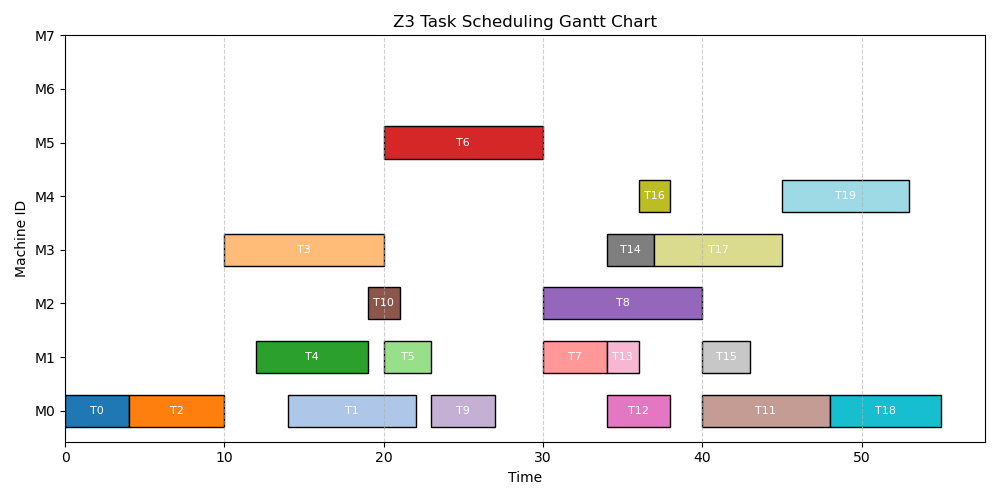
\includegraphics[width=0.8\textwidth]{7a.png} 
    \caption{Task scheduling Gantt chart (before optimization).} 
    \label{fig:gantt} 
\end{figure}
\begin{figure}[h] 
    \centering
    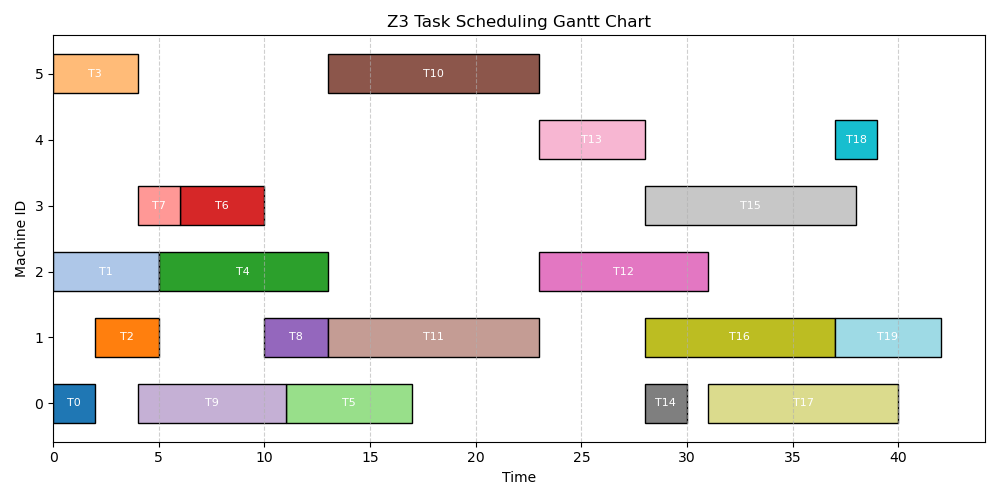
\includegraphics[width=0.8\textwidth]{7a_opt.png} 
    \caption{Task scheduling Gantt chart (after optimization).} 
    \label{fig:gantt} 
\end{figure}

\subsection{Solver Performance}
\begin{itemize}
    \item Initially, the total runtime is 47.462405 seconds.
    \item After optimization, the total runtime is 1.649142 seconds.
    \item In conclusion, the optimized version saves 96.52\% of time.
\end{itemize}


\end{document}